
It's not always possible to use derivative in order to optimize a
fonction with a continuous domain because:
\begin{enumerate}
    \item  The gradient is not computable
    \item  We dont know the objective function
    \item  The gradient is to expensive to compute
    \item  We don't know how to compute the gradient
\end{enumerate}

In this case, we can use \textbf{Derivative free optimization}.
We dont know the objective function but we have comparison function that allows us to compare solutions.


\subsection{Background}
%TODO

\subsection{Grid Search}

As the domain is continuous and we can't compare every point:
\begin{enumerate}
    \item Cut each dimension of the domain $\Omega$ in m
    \item Evaluate each one of these combination 
    \item Output the minimum

    \item[$\Rightarrow$]  We will always have $m^n$ evaluation,
        because we have $n$ dimensions that
we cut in $m$ parts.
\end{enumerate}

\subsubsection{Iteratively}
\begin{itemize}
    \item Perform a grid search for the domain $\Omega$ 
    \item Around the min point found define a new smaller domain
        $\Omega$ 
    \item[$\Rightarrow$] So if we do i iterations we will have $i *
        m^n$ evaluations for the objective.
\end{itemize}

\subsection{Directional Direct Search}

\begin{tabular}{m{12cm}m{3cm}}
The global idea is to \textbf{test a sample of points} in specified
directions around the iterate.
If a point is better, select it as next iterate.
&

\includegraphics[width=2cm]{DDS}
\end{tabular}

\subsubsection{Step}

\begin{enumerate}
    \item \textbf{Poll step}: Test $N$ points in specified directions
        around iterate and stop when better (with our comparison
        function) point found.

        \begin{itemize}

            \item \textbf{Directions and bases}
                We define a set $D$ of positive bases used to evaluate new
                points (directions):
                $$D = [l, -l] = [e_1,..., e_n, -e_1,..., -e_n]$$
                where the $e_i (1 < i < n)$ are unit vector ($||e_i|| = 1$)

            \item \textbf{Build new point}: 
                $$x_(new) = x+\alpha*d \quad \textrm{where } d \in D$$
        \end{itemize}

        \paragraph{Example} For a 3D space,
        $$D = [l, -l] = [e_1, e_2, e_3, -e_1, -e_2, -e_3] \quad
        \textrm{where} \quad \begin{cases}
            e_1 = (1,0,0) \\
            e_2 = (0,1,0)\\
            e_3 = (0,0,1)\\
        \end{cases} $$
        $$\textrm{Suppose} \quad \begin{cases} 
            x = (40, 42, 42)\\
            d = (1, 0, 0)\\
            \alpha =2
        \end{cases} \quad           
        x_{new}  = (40, 42, 42) + 2 * (1, 0, 0) = (42, 42, 42)$$


    \item \textbf{Mesh parameter update}: Update or maintain the step
        size parameter, $\alpha_k$ in order to converge faster.

        \begin{enumerate}
            \item Iteration declared successful: increase $\alpha_k$ to
                perform greater step
                $$\alpha_{k+1} = \gamma \alpha_k \quad \textrm{with}\quad \gamma > 1$$

            \item Iteration declared unsuccessful: decrease $\alpha_k$ to
                converge to an optimum
                $$\alpha_{k+1} = \beta \alpha_k \quad \textrm{with}\quad
                0 < \beta < 1$$
            \end{enumerate}
\end{enumerate}

\subsubsection{Denis-Wood Coutours}

\begin{tabular}{m{12cm}m{5cm}}
No convergence if Denis-Wood contours appears in objective
function
&
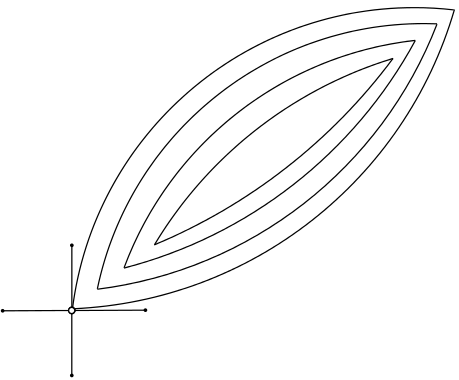
\includegraphics[width=2cm]{contour}
\end{tabular}

\paragraph{Two solutions}:
\begin{enumerate}
    \item Rotate the bases after $N$ unsuccessful iterations
    \item Run DDS $N$ times with $N$ different set of bases.
    \end{enumerate}

\subsubsection{One iteration complexity}
\begin{itemize}
    \item Worst case: $Nb_{evals} = 2b = 0(b)$ where $b$ is the number
        of bases used
    \item Best case: $Nb_{evals} = 1 = \Omega(1)$
\end{itemize}


\subsection{The Nelder-Mead Algorithm}

The global idea is to build a structure of points and replace the worst
point at each iteration.

\subsubsection{Simplex}
\begin{tabular}{m{12cm}m{3cm}}
    \begin{itemize}
        \item The structure of point is a polyhedron of dimension $n+1$
            (abusively called simplex)

    \item The simplex structure $Y$ is a set of $n+1$ vertices where $n$ is the
dimension of the search space defined as follows:
$$Y = \{y^0,y^1,...,y^n\}$$

\item The vertice $y^0$ is a better solution than the vertice $y^1$ which is a better solution that then vertice $y^2$ ....
        \end{itemize}
&
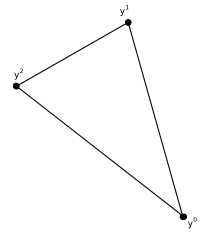
\includegraphics[width=3cm]{polyhedron}
\end{tabular}

\subsubsection{Operations on the simplex}
At each iteration, replace the worst point by performing one of the
following actions:
\begin{enumerate}
    \item \begin{tabular}{m{9cm}m{3cm}}
            \textbf{Reflection} if $f^0 \leq f < f^{n-1}$ : Replace $y^n$ by $y^r$

            $$Nb_{evals} = 1 = \Theta(1)$$
            & 
            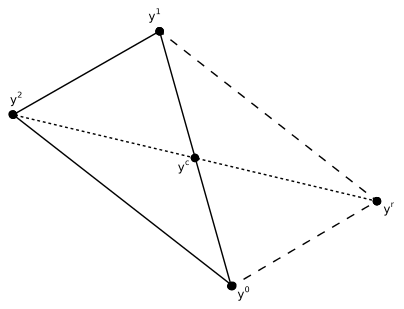
\includegraphics[width=4cm]{reflection}
        \end{tabular}

    \item \begin{tabular}{m{9cm}m{3cm}}
            \textbf{Expansion} if $f^r < f^0$ : 
            \begin{itemize}
                \item If $f^e \leq f^r$ replace $y^n$ by $y^e$
                \item else replace $y^n$ by $y^r$
            \end{itemize}

            $$Nb_{evals} = 2 = \Theta(1)$$
            & 
            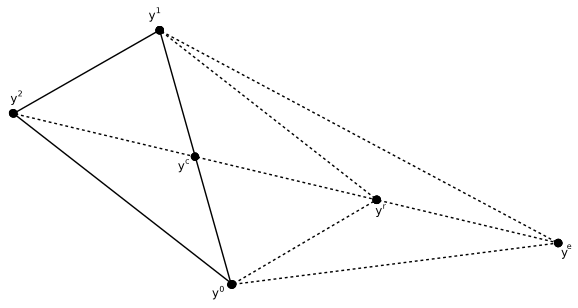
\includegraphics[width=4cm]{expansion}
        \end{tabular}

    \item \begin{tabular}{m{9cm}m{3cm}}
            \textbf{Contraction} if $f^r \geq f < f^{n-1}$ : 
            \begin{itemize}
                \item If $f^r < f^n$ replace $y^n$ by $y^{oc}$ (outside)
                \item else replace $y^n$ by $y^{ic}$ (inside)
            \end{itemize}

            $$Nb_{evals} = 2 = \Theta(1)$$
            & 
            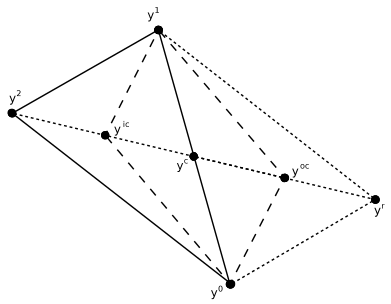
\includegraphics[width=4cm]{contraction}
        \end{tabular}

    \item \begin{tabular}{m{9cm}m{3cm}}
            \textbf{Shrink} if no amelioration by doing thos 

            $$Nb_{evals} = n+2 = \Theta(n)$$ where $n$ is the dimension
            of the search space
            & 
            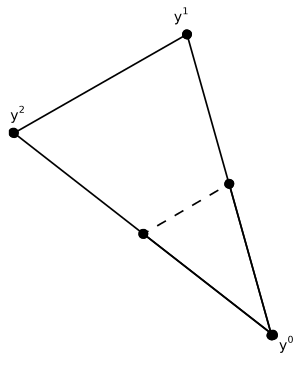
\includegraphics[width=4cm]{shrink}
        \end{tabular}
\end{enumerate}


\subsection{Multi-Directional Search}
Global idea\newline
Same point structure than in Nelder-Mead.\newline
Perform operations on all but one vertices of the simplex around
the best vertex.\newline
The point structure\newline
\newline
The structure of point is a polyhedron of dimension n + 1 (The
simplex of Nelder-Mead).\newline

\subsubsection{Operations on the simplex}
1)Rotation\newline
2)Expansion\newline

Rotation\newline
Evaluate $f^r = min{f(y^r_i)|i=,;...;n}$\newline
if $f^r$ < $f^0$ -> expansion\newline
else -> contract simplex \newline

Expansion\newline
Evaluate $f^r = min{f(y^r_i)|i=,;...;n}$\newline
if $f^e$ < $f^r$ -> The new simplex is the expanded simplex\newline
else -> cThe new simplex is the rotated simplex \newline

Shrink\newline

\subsubsection{Complexity}
Rotation\newline
O(n)\newline
Expansion\newline
O(n)\newline
Shrink\newline
O(n)

\subsection{Smart Random Algorithms}
Problem:\newline
Algorithm might converto to local minimum.\newline
Solution\newline
Restart from different points\newline

Idea:\newline
Run  N times the algirithm such as:\newline
1)For each run the algorithm begins from a random starting
point\newline
2)Random starting points following a uniform distribution\newline
3)Return the best result obtained over the N runs\newline

Problem is that those random sequence might contain gaps.\newline
To avoid that problem we use Halton Sequence.\newline
How to build a Halton sequence:\newline
Chose a base(integer) and successively decompose [0, 1] in subintervals according to the base.\newline

To build multi dimensional Halton sequence we build n 1D qequence with n different bases(prime two by two) and we mix the points.\newline
Problem with higher prime sequence (correlation problem).\newline
Solution:\newline
Shuffle one of the sequence before mixing the different sequence to build the points
